
\subsection{Datasets}
\begin{table}
\resizebox{1\columnwidth}{!}{
\begin{tabular}{ll|cc|c}
Language&&Size (MB)&Tokens (M)& Sentences (K)\\
\toprule 
Bulgarian&BG&36.11&8.53&329\\
Czech&CS&53.48&12.25&535\\
German&DE&171.80&44.07&1785 \\
English&EN&179.15&49.32&1815\\
Finnish&FI&145.32&32.85&1737\\
French&FR&197.68&53.82&1792\\
Hungarian&HU&52.53&12.02&527\\
Italian&IT&186.67&48.08&1703\\
Portuguese&PT&187.20&49.03&1737\\
\end{tabular}}
\caption{Data statistics after tokenizing, sentence-splitting, and removing markups, and numberizing. Tokens and sentence counts refer to the training partition. \trevor{Move to \supp}}
\end{table}

\begin{figure}
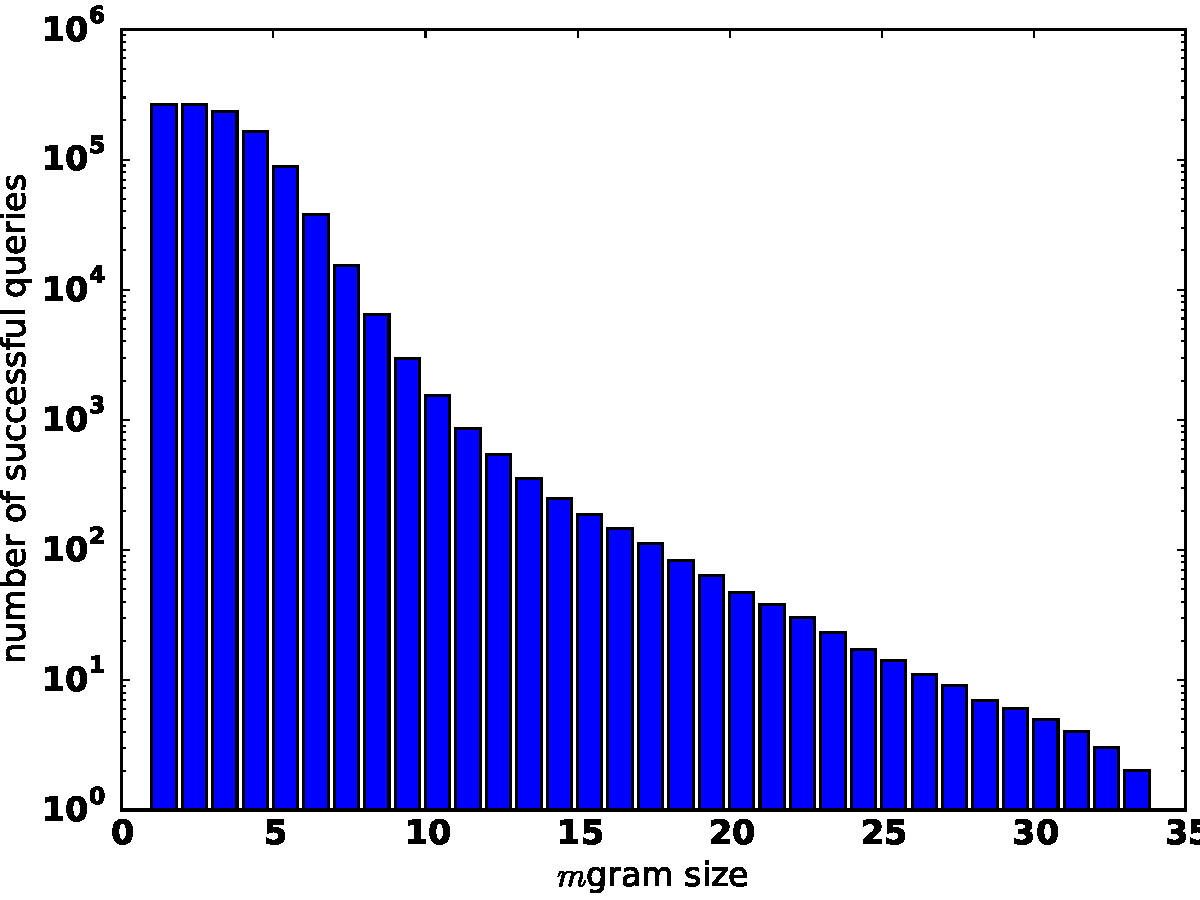
\includegraphics[width=\columnwidth]{figures/german_pattern_size.pdf}
\caption{Number of successful queries across different pattern sizes from KN computation over the German test set, with unbounded $m$.}
\end{figure}

\missingfigure[figwidth=\columnwidth]{All 9 languages pplx results with m=2..10,15,20,infinity.}

\missingfigure[figwidth=\columnwidth]{On German, showing the size in MB (y axis) and time (x axis) for 4 methods: CST single, CST dual, SRILM, SRILM compact. Each method is a 'line' connecting m=2,3,4,... Only CST single will go beyond m=6.}

\missingfigure[figwidth=\columnwidth]{Wikipedia pplx (right axis), and time (left axis) for the single CST on characters vs words as a function of \ngram size.}

\missingfigure[figwidth=\columnwidth]{Wikipedia histogram over \ngram size, perhaps as a figure or table?}

\missingfigure[figwidth=\columnwidth]{Wikipedia plot (stacked bar?) of time spent in each method (n1+ x 3; backward search etc) as a function of n.}

% \begin{table*}\footnotesize
% \centering
% \begin{tabular}{llllllll|llll|llll}
% \toprule 
% & & \multicolumn{6}{c}{KenLM - ModifiedKN} & \multicolumn{4}{c}{SRILM - KN} & \multicolumn{4}{c}{CST - KN}\\
% & & \multicolumn{2}{c}{probing}& \multicolumn{2}{c}{trie}& \multicolumn{2}{c}{compact trie}& \multicolumn{2}{c}{default} & \multicolumn{2}{c}{compact} &\multicolumn{2}{c}{Dual}& \multicolumn{2}{c}{Single}\\
%  \midrule
% &&MB&Sec&MB&Sec&MB&Sec&MB&Sec&MB&Sec&MB&Sec&MB&Sec\\
%       \midrule
% \multirow{3}{*}{BG} 
%  & n=2 &&&&&&&&&&&&&&\\
%  & n=3 &&&&&&&&&&&&&&\\
%  & n=4 &&&&&&&&&&&&&&\\
%  & n=8 &&&&&&&&&&&&&&\\
%  & n=9 &&&&&&&&&&&&&&\\
%  & n=10 &&&&&&&&&&&&&&\\\hline
%  \multirow{3}{*}{CS}
%  & n=2 &&&&&&&&&&&&&&\\
%  & n=3 &&&&&&&&&&&&&&\\
%  & n=4 &&&&&&&&&&&&&&\\
%  & n=8 &&&&&&&&&&&&&&\\
%  & n=9 &&&&&&&&&&&&&&\\
%  & n=10 &&&&&&&&&&&&&&\\\hline
%  \multirow{3}{*}{DE}
%  & n=2 &&&&&&&&&&&&&&\\
%  & n=3 &&&&&&&&&&&&&&\\
%  & n=4 &&&&&&&&&&&&&&\\
%  & n=8 &&&&&&&&&&&&&&\\
%  & n=9 &&&&&&&&&&&&&&\\
%  & n=10 &&&&&&&&&&&&&&\\\hline 
%  \multirow{3}{*}{EN} 
%  & n=2 &&&&&&&&&&&&&&\\
%  & n=3 &&&&&&&&&&&&&&\\
%  & n=4 &&&&&&&&&&&&&&\\
%  & n=8 &&&&&&&&&&&&&&\\
%  & n=9 &&&&&&&&&&&&&&\\
%  & n=10 &&&&&&&&&&&&&&\\\hline 
%  \multirow{3}{*}{FI}
%  & n=2 &&&&&&&&&&&&&&\\
%  & n=3 &&&&&&&&&&&&&&\\
%  & n=4 &&&&&&&&&&&&&&\\
%  & n=8 &&&&&&&&&&&&&&\\
%  & n=9 &&&&&&&&&&&&&&\\
%  & n=10 &&&&&&&&&&&&&&\\\hline 
%  \multirow{3}{*}{FR}
%  & n=2 &&&&&&&&&&&&&&\\
%  & n=3 &&&&&&&&&&&&&&\\
%  & n=4 &&&&&&&&&&&&&&\\
%  & n=8 &&&&&&&&&&&&&&\\
%  & n=9 &&&&&&&&&&&&&&\\
%  & n=10 &&&&&&&&&&&&&&\\\hline 
%  \multirow{3}{*}{HU}
%  & n=2 &&&&&&&&&&&&&&\\
%  & n=3 &&&&&&&&&&&&&&\\
%  & n=4 &&&&&&&&&&&&&&\\
%  & n=8 &&&&&&&&&&&&&&\\
%  & n=9 &&&&&&&&&&&&&&\\
%  & n=10 &&&&&&&&&&&&&&\\\hline
%  \multirow{3}{*}{IT}
%  & n=2 &&&&&&&&&&&&&&\\
%  & n=3 &&&&&&&&&&&&&&\\
%  & n=4 &&&&&&&&&&&&&&\\
%  & n=8 &&&&&&&&&&&&&&\\
%  & n=9 &&&&&&&&&&&&&&\\
%  & n=10 &&&&&&&&&&&&&&\\\hline 
%  \multirow{3}{*}{PT}
%  & n=2 &&&&&&&&&&&&&&\\
%  & n=3 &&&&&&&&&&&&&&\\
%  & n=4 &&&&&&&&&&&&&&\\
%  & n=8 &&&&&&&&&&&&&&\\
%  & n=9 &&&&&&&&&&&&&&\\
%  & n=10 &&&&&&&&&&&&&&\\
%      \bottomrule
% \end{tabular}
% \caption{Memory and Space consumption during kenlm and srilm training, and buidling the CST.}
% \end{table*}
% \begin{table*}\footnotesize
% \centering
% \begin{tabular}{lllllllll|lllll|lllll}
% \toprule 
% & & \multicolumn{7}{c}{KenLM - ModifiedKN} & \multicolumn{5}{c}{SRILM - KN} & \multicolumn{5}{c}{CST - KN}\\
% & & \multicolumn{2}{c}{probing}& \multicolumn{2}{c}{trie}& \multicolumn{2}{c}{compact trie}& \multicolumn{1}{c}{pplx} & \multicolumn{2}{c}{default} & \multicolumn{2}{c}{compact} &\multicolumn{1}{c}{pplx} &\multicolumn{2}{c}{Dual}& \multicolumn{2}{c}{Single}& \multicolumn{1}{c}{pplx}\\
%  \midrule
% &&MB&Sec&MB&Sec&MB&Sec&&MB&Sec&MB&Sec&&MB&Sec&MB&Sec&\\
%       \midrule
% \multirow{3}{*}{BG} 
%  & n=2 &&&&&&&&&&&&&&&&&\\
%  & n=3 &&&&&&&&&&&&&&&&&\\
%  & n=4 &&&&&&&&&&&&&&&&&\\
%  & n=8 &&&&&&&&&&&&&&&&&\\
%  & n=9 &&&&&&&&&&&&&&&&&\\
%  & n=10 &&&&&&&&&&&&&&&&&\\\hline
%  \multirow{3}{*}{CS}
%  & n=2 &&&&&&&&&&&&&&&&&\\
%  & n=3 &&&&&&&&&&&&&&&&&\\
%  & n=4 &&&&&&&&&&&&&&&&&\\
%  & n=8 &&&&&&&&&&&&&&&&&\\
%  & n=9 &&&&&&&&&&&&&&&&&\\
%  & n=10 &&&&&&&&&&&&&&&&&\\\hline
%  \multirow{3}{*}{DE}
%  & n=2 &&&&&&&&&&&&&&&&&\\
%  & n=3 &&&&&&&&&&&&&&&&&\\
%  & n=4 &&&&&&&&&&&&&&&&&\\
%  & n=8 &&&&&&&&&&&&&&&&&\\
%  & n=9 &&&&&&&&&&&&&&&&&\\
%  & n=10 &&&&&&&&&&&&&&&&&\\\hline 
%  \multirow{3}{*}{EN} 
%  & n=2 &&&&&&&&&&&&&&&&&\\
%  & n=3 &&&&&&&&&&&&&&&&&\\
%  & n=4 &&&&&&&&&&&&&&&&&\\
%  & n=8 &&&&&&&&&&&&&&&&&\\
%  & n=9 &&&&&&&&&&&&&&&&&\\
%  & n=10 &&&&&&&&&&&&&&&&&\\\hline 
%  \multirow{3}{*}{FI}
%  & n=2 &&&&&&&&&&&&&&&&&\\
%  & n=3 &&&&&&&&&&&&&&&&&\\
%  & n=4 &&&&&&&&&&&&&&&&&\\
%  & n=8 &&&&&&&&&&&&&&&&&\\
%  & n=9 &&&&&&&&&&&&&&&&&\\
%  & n=10 &&&&&&&&&&&&&&&&&\\\hline 
%  \multirow{3}{*}{FR}
%  & n=2 &&&&&&&&&&&&&&&&&\\
%  & n=3 &&&&&&&&&&&&&&&&&\\
%  & n=4 &&&&&&&&&&&&&&&&&\\
%  & n=8 &&&&&&&&&&&&&&&&&\\
%  & n=9 &&&&&&&&&&&&&&&&&\\
%  & n=10 &&&&&&&&&&&&&&&&&\\\hline 
%  \multirow{3}{*}{HU}
%  & n=2 &&&&&&&&&&&&&&&&&\\
%  & n=3 &&&&&&&&&&&&&&&&&\\
%  & n=4 &&&&&&&&&&&&&&&&&\\
%  & n=8 &&&&&&&&&&&&&&&&&\\
%  & n=9 &&&&&&&&&&&&&&&&&\\
%  & n=10 &&&&&&&&&&&&&&&&&\\\hline
%  \multirow{3}{*}{IT}
%  & n=2 &&&&&&&&&&&&&&&&&\\
%  & n=3 &&&&&&&&&&&&&&&&&\\
%  & n=4 &&&&&&&&&&&&&&&&&\\
%  & n=8 &&&&&&&&&&&&&&&&&\\
%  & n=9 &&&&&&&&&&&&&&&&&\\
%  & n=10 &&&&&&&&&&&&&&&&&\\\hline 
%  \multirow{3}{*}{PT}
%  & n=2 &&&&&&&&&&&&&&&&&\\
%  & n=3 &&&&&&&&&&&&&&&&&\\
%  & n=4 &&&&&&&&&&&&&&&&&\\
%  & n=8 &&&&&&&&&&&&&&&&&\\
%  & n=9 &&&&&&&&&&&&&&&&&\\
%  & n=10 &&&&&&&&&&&&&&&&&\\
%      \bottomrule
% \end{tabular}
% \caption{Memory and Space consumption during the query time, and the perplexities}
% \end{table*}

\subsection{Perplexity Evaluation}




%%% Local Variables: 
%%% mode: latex
%%% TeX-master: "cstlm"
%%% End: 
